\clearpage % Rozdziały zaczynamy od nowej strony.

\section{Motivation}

\subsection{Digital Preservation}

The Digital Preservation is a pursuit to conserve both content which was
reformatted to digital and information which was born-digital, that is, which
originated in the digital form. While the goals are quite similar to the
standard archival practices, the challenges, techniques, and technologies used
are quite different.

It might seem that preserving something digital would be much easier than
preserving something that is physical, considering that in the case of
a digital entity mere passage of time does not corrupt it and that it is
trivial to create perfect copies that are as authentic as the original. This is
not necessarily the case. While physical artefacts decay from exposure to
moisture, heat, cold, oxygen, light etc. the digital is wholly reliant on its
environment - the hardware and software that is used to preserve it and present
it. These hardware parts are exposed to and affected by the elements in the
same way a book or an art piece is. These can lead to bit rot - the corruption
of data caused by loss of charge or loss of magnetic orientation in solid state
media or in magnetic media, and by breakdown of the optical media. What is
more, the rest of the hardware used is highly complex and might experience
unpredictable failure whose probability increases with time. Some of these
problems can be solved in software, some are solved by using specialised
hardware for the purpose of archiving, which can mitigate the corruption of
data and extend its lifetime. The problem with these is that most of such
products are proprietary. Companies that create and provide support for them
can go bankrupt, lose patents or stop providing the technology required for
other reasons. Finally the digital resources are susceptible to events that
would not affect properly stored physical heritage, like eg. a geomagnetic
storm that could wipe digitally stored data but would not be dangerous to
physical objects.

Another consideration when it comes to digital materials is that they contain
only the ``immediate'' information while physical objects carry much more
additional information that allows to study their context. The digital by
itself carries only intended data: a book only offers the text, a movie,
a picture, or a piece of music only provides what it has on its own. A physical
book or an art piece offers much more: the materials can be studied, the
texture or a font can be analysed. Inspecting a physical artefact makes it
possible to discover its journey. This makes the process of authenticating and
ensuring that a digital piece was not modified so difficult and so much
different than a physical one. This is also why it is needed to keep a spurious
amounts of metadata about digital objects.

The difficulty with preserving digital records is even greater with data that
is not ``static'' but rather ``interactive'' like software. Conversion from an
older file format to a new one that has better support or is better equipped
for use in archiving is infinitely less difficult of an endeavour than
ensuring that a piece of software is operational over the years. In general
there are two strategies to provide sustained accessibility to digital
objects: migration and emulation \cite{hoeven2007}. Migration concerns the
digital object itself in changing the object in such a way that it is possible
to render the original object despite developments of the underlying software
and hardware environment used for preservation. In the case of ``static'' data
the migration would be to convert the files to a newer file format, whereas
for a ``dynamic'' digital object it would have to be ported i.e. rewritten to be
compatible with the newer software or hardware. That is almost always pretty
much impossible when dealing with proprietary objects where the source code is
missing, and when the source code is available it is still a monumental
undertaking. Emulation on the other hand deals with changing the environment
or providing a compatibility layer that would allow for sustained
accessibility of the unchanged object by recreating an equivalent of its
original environment.

Emulation in itself is a really complicated problem. It requires simulation of
lots of ``moving parts'' and the system being emulated is often not well
documented or not documented at all. This makes the process of creating an
emulation environment a process of trial and error, and there is never
a guarantee that something does not break because it dependent on some
undocumented, undiscovered behavior. There are a few approaches to emulation.
One is creating a ``thin'' compatibility layer, that is providing stubs for
missing pieces and adaptors for existing features that are different. Such
a solution can work for example for running software created for the same or
similar computer architecture but on a different operating system, it is what
WiNE is doing to run Windows programs on Linux. Another approach is to simulate
a complete computer. This is much more complex and demanding but allows for
cross platform emulation - software and operating systems meant for one type of
device and be run through emulation on a device with a completely different
architecture. There are also solutions that combine emulation of hardware with
emulation of the operating system, like DOSBox which both emulates computer
hardware and provides a DOS environment. This kind of approach can provide
better compatibility but is less flexible. Using these types of tools is
a great starting point in the project of archiving software. In fact the
archive.org organisation provides a Windows 95 environment that runs inside
a browser and is available on the organisation's website \cite{win95web} by
using a slightly modified version of DOSBox compiled using Emscripten,
a compiler that allows compiling C or C++ software for browsers. However, it is
not enough, none of these tools was built with long term digital preservation
in mind \cite{hoeven2007}.

\subsection{What is PenPoint OS}

Released in 1991 PenPoint was an operating system that was created with devices
that were truly mobile in mind. The creators of PenPoint saw the need for
a device with the functionality of a computer that could be used on the move.
They noticed that laptops, although touted as mobile, were actually just
movable desktop computers. What they had in mind were devices that did not have
to be set up on a desk or a lap, but one you could take from meeting to meeting
\cite{startupadv} without any hassle or even operate with one hand and holding
it with the other while walking \cite{carr1991}. Something like today's
smartphone but in many ways different. They understood that such a computer
could not be just a smaller lighter PC but designed from the ground up with
these requirements in mind.

\subsection{Brilliance of PenPoint}
PenPoint is built around three main ideas: the Notebook User Interface (NUI)
metaphor, the Embedded Document Architecture (EDA), and the focus on
connectivity. All of those are tightly interconnected and provide a complete
and well designed coherent environment.

The NUI is a user interface metaphor that is much better suited for a mobile
portable system than a desktop metaphor. The NUI is present all throughout the
system. The most important part of the NUI is the notebook itself, it takes the
vast majority of the screen. Below the notebook there is the ``bookshelf'', and
above there is a menu bar that can be turned off when the user is more familiar
with how to use PenPoint OS in the idiomatic way of using gestures for most of
the tasks. The bookshelf is a meta-area that stores notebooks and other
systemwide objects and resources, such as the help notebook, disk manager, and
in and out boxes. The menu bar contains the familiar dropdown menus with
editing functionality \ref{fig:notebook-user-interface1}.

\begin{figure}[!h]
    \centering 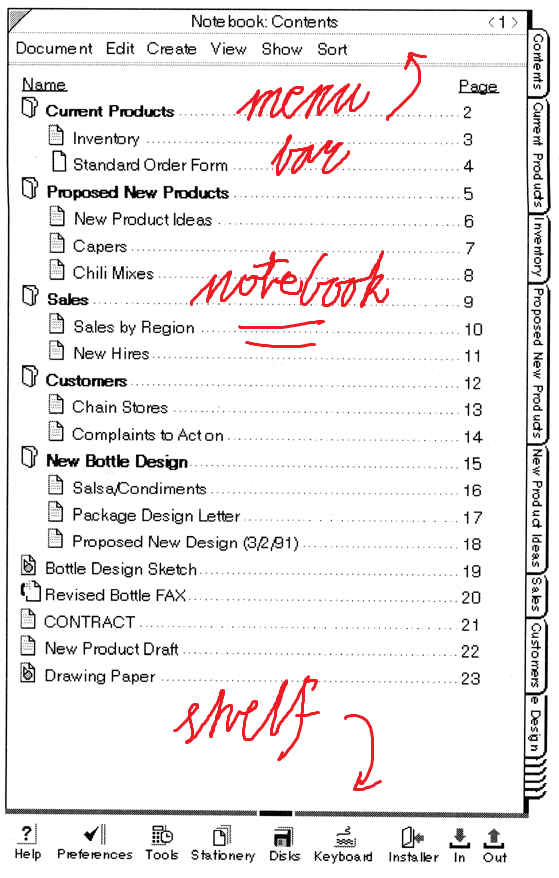
\includegraphics[width=0.5\linewidth]{penpoint-interface-1.png}
    \caption{PenPoint OS: Notebook User Interface}
    \label{fig:notebook-user-interface1}
\end{figure}

The notebook consists of a table of contents in the middle, tabs on the right
that simulate tabs such as those in a three-ring binder, and an optional ``cork
margin'' at the bottom \ref{fig:notebook-user-interface2}. The table of contents
is where all user data is organised. Each document is presented as a page in
the summary. Pages might also be grouped into sections, and sections can be
nested as well which allows creation of hierarchies similar to directories and
files. Each document is also analogous to a program, this is a part of the EDA.
The tabs allow to jump instantly to a page or a section in the notebook.
PenPoint also allows programs to use tabs for their internal navigation.

\begin{figure}[!h]
    \centering 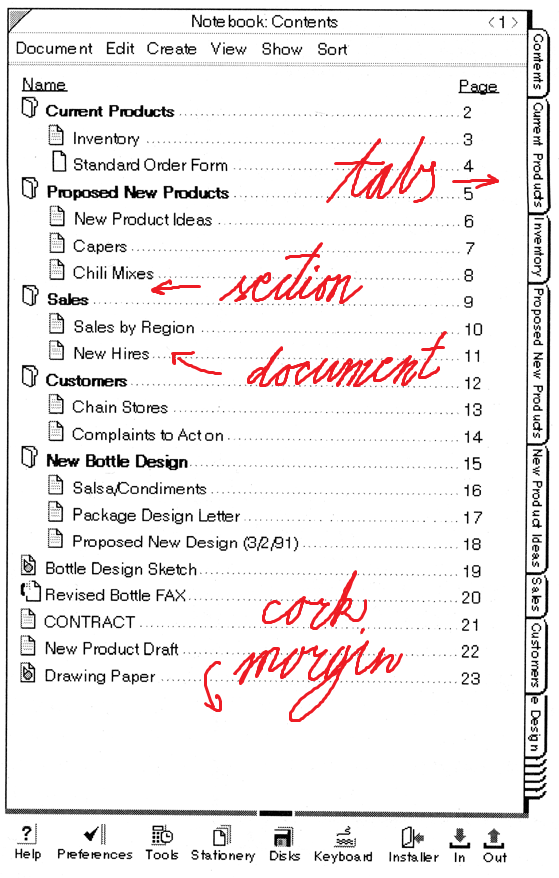
\includegraphics[width=0.5\linewidth]{penpoint-interface-2.png}
    \caption{PenPoint OS: Notebook User Interface}
    \label{fig:notebook-user-interface2}
\end{figure}

The ``cork margin'' is a place attached to the bottom of any document frame that
can contain any PenPoint object \ref{fig:cork-margin}. It is named that because
you can ``pin'' things there as on a cork board. It is turned off by default.

\begin{figure}[!h]
    \centering 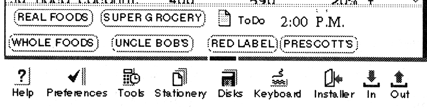
\includegraphics[width=0.5\linewidth]{cork-margin.png}
    \caption{PenPoint OS: Cork Margin}
    \label{fig:cork-margin}
\end{figure}

In Embedded Document Architecture every file is also equivalent to an instance
of a program. Clicking a page opens up the file in the associated application,
there is no distinction between them. There is no notion of saving or loading
\cite{startupadv}, everything is always ready to go. This is what a document is
in PenPoint \cite{carr1991} \cite{brown1992}. But a more important and
impressive aspect of EDA is the ``embedded'' part. In PenPoint every document
has the ability to embed every other document, and this nesting can go as far
as the hardware is capable of. This goes from simple stuff like writing pads
\ref{fig:embedded-document-architecture} - areas that are used for text input,
that could be of different sizes, floating or docked, with input fields
separated into cells or continuous, or signature pads - to things like
pluggable spellcheck or even to embedding a whole drawing program inside of
a presentation for example.  EDA also allows to copy any and all objects from
one document to another without any loss of quality or information
\cite{carr1991} \cite{brown1993}. In PenPoint the gestures are global and
present all throughout; however it is up to the ``surface'' gesture was issued
on to decide what it means. Inside a writing pad it is interpreted as a letter,
whereas in a drawing document it could be either interpreted as a shape or an
editing gesture: delete, select, etc. The embedding was not only a useful
functionality but it also created a greater code reuse and thus lowered the
hardware requirements.

\begin{figure}[!h]
    \centering 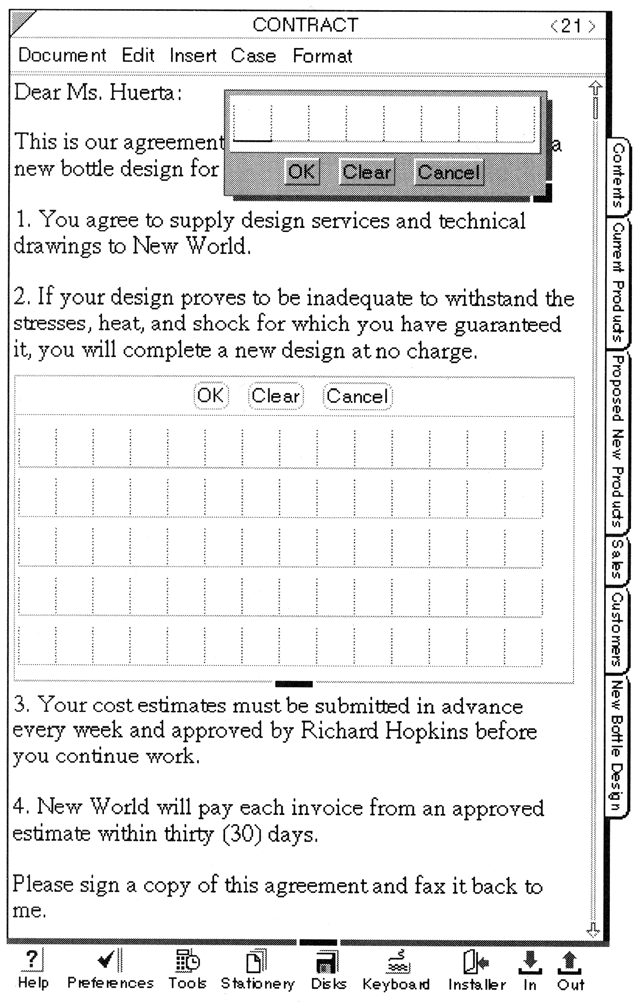
\includegraphics[width=0.5\linewidth]{penpoint-interface-3.png}
    \caption{PenPoint OS: Embedded Document Architecture - writing pads}
    \label{fig:embedded-document-architecture}
\end{figure}

The third main idea is the focus on connectivity. One of the goals of PenPoint
was to be as compatible with different communication protocols as possible.
This meant internet and email but also printers and faxes, it also included not
having to restart the computer in order to connect to a new network which was
not always the case with other devices at the time. Being able to receive fax
on a PenPoint device meant that it was possible to add freehand notes and
drawings to the received image and resend it without any loss of quality, and
without having to print it and scan it \cite{godemo1991}. The focus on
connectivity also manifested itself in the global address book and an unified
inbox and outbox present in PenPoint. One innovative feature of the PenPoint
outbox was delayed I/O. The delayed I/O was a functionality whereby it was
possible to write and ``send'' an email without a need for internet connection,
with the system scheduling the message to be actually sent when the connection
was present again \cite{carr1991} \cite{brown1993}.

Although I would consider them to be a part of NUI gestures \ref{fig:gestures}
deserve special attention. What made them so powerful is the fact that
a gesture specifies both the target and the command given - crossing out a word
applies the delete operation on that word, crossing out a shape deletes the
shape. Because of this it was important to provide a lot of gestures and make
them work seamlessly. Gestures and their recognition were implemented on
a system level but it was up to the program to interpret a gesture and act on
it. PenPoint provides about a dozen core gestures that work uniformly across
all the apps with common commands, so a delete or edit gesture would work just
as well on a word, a drawn object or a calendar entry.  Additionally, there are
many more gestures that were application specific.

\begin{figure}[!h]
    \centering 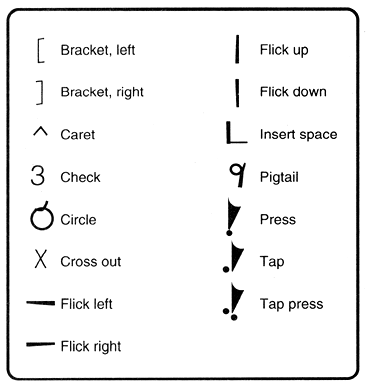
\includegraphics[width=0.5\linewidth]{gestures.png}
    \caption{PenPoint OS: Gestures}
    \label{fig:gestures}
\end{figure}

Nowadays there is lesser interest in a compelling user interface metaphor.
Instead the metaphors encompass only a small portion of the whole, and the
designs are becoming more self-referential - they rely on the familiarity with
the previous versions or similar environments rather than something universal.
Although a smartphone with a touch screen is probably the most popular device
the use of gestures is minimal, other than simple swipes to go back and switch
between applications, and the extremely powerful notion of target and command
that a gesture provides is non-existent. Some applications, especially centred
around phones employ the PenPoint idea of a document where the data and the
program go hand in hand, and there is no loading or saving. And some even try
to do the embedding part, but the embedding is usually very much limited
compared to what was possible in PenPoint, and requires additional resources
because it is not supported on the system level. Features like unified inbox
and delayed I/O are also missing from modern devices. Some programs have
similar concepts but without inbuilt system support these functionalities just
can not reach full potential, and even though a reliable connection is almost
always available there is still 1\% of situations where delayed I/O would be
incredibly useful.

\subsection{PenPoint OS: Too great a vision}

PenPoint OS failed. It did not become successful and today is mostly forgotten,
even though a great deal of its original features are still used in today's
operating systems, and many are still missing or unmatched in capability to
ones PenPoint offered. A large set of gestures that worked system-wide and
``press and hold'' for any selection, a dynamic layout toolkit which allowed
applications to automatically rescale for portrait or landscape orientation,
a global pluggable address book and support for as many connection standards as
possible, as well as automatic scheduling of operations that required
connection for when that connection would be established, like sending or
receiving emails, a document architecture where each document was an instance
of a program and each document could nest another document. All of these were
either innovated or advanced by PenPoint. PenPoint OS was extremely well
designed with the pen-centricity and mobility in mind, and it was coherent in
that design. The notebook interface metaphor was present throughout the whole
user interface.

Despite all of this PenPoint OS did not gain adoption. The biggest and most
obvious problem was the hardware available at the time. Even though the
developers employed many clever solutions and tricks that allowed PenPoint to
operate on a variety of different computers and scale with the available
resources the problem that could not be overcome was that the technology
required just was not there back then - the screens were dim and low resolution,
the latency was high and the handwriting recognition was not up to par. Even
now, after over 30 years of rapid hardware evolution and incredible leaps in
technology later with resolutions so high and latencies so low that pixels and
delays are virtually imperceivable, writing on a digital device feels off to
many people. In spite of countless advantages offered by the digital, the
feeling of pen and paper still feels superior.

\subsection{Evolution of graphical interfaces: looking back to move forward}

The advancements in graphical user interfaces seem to not be able to keep up
with the ever growing complexities of the software. In fact apart from
aesthetic stylistic changes there is not a lot of change at all, and in some
aspects it could be argued that GUIs are regressing. The proceeding unification
of interfaces across the web and desktop applications and computers, tablets,
and smartphones makes it easier for developers to create new software and for
the users to become familiar with it, but makes it impossible to use any of the
domains to the fullest. In almost all cases a non-graphical or mix of graphical
representation and non-graphical input provides greater possible speed. That's
why many professionals still use text based interfaces or opt for workflows
relying heavily on keyboard shortcuts. The advantages of graphical user
interfaces used to be ease of use and discoverability. This, however, slowly
begins to be less and less the case - with applications being more and more
advanced and providing more and more features the cascading menus become more
and more crammed and overloaded, and thus less welcoming. The use of gestures
had a little bit of a resurgence with the adoption of bigger touchpads and
touch sensitive screens in laptops. These unfortunately often work only at
a system level or are not uniformly supported across applications. The most
widely used alternative form of input are voice commands. Voice control
unfortunately is only useful at times when any other method is not possible or
not easily accessible like operating navigation while driving or smart home
without moving from the couch. It is not adequate for use in the office or in
loud public places.

As it often happens in engineering, good ideas, sometimes brilliant ideas are
discarded and forgotten because they are held back by the technology available.
And sometimes an entire approach to a problem is rejected as wrong. But then
the knowledge and state of the art changes and these ideas and approaches have
to be discovered all over again. That is why knowing past solutions and looking
there for current and future solutions can yield great results. Those who do
not know the history are bound not to remember that one thing that someone else
did that one time and it did not work but might work now.

